Processes are designed to limit bad behavior or to allocate scarce resources


\gls{process}

Processes improve scalability. Cite the pin factory example

Processes to address risk. These involved justification

Processes to improve consistency

Processes to enable specialization

Processes change over time because the conditions change. Processes are implemented differently than intended because the people implementing them are not the same people who came up with and designed them
*********************
New people are likely to arrive and ask what are the processes and where is the documentation?

People have been on a team for a long time say don't burden me with processes I just need to get things done using the relationships with the people I have.


In addition to not having formed a social network, there's a second reason new people seek processes.

Recently graduated people from school are used to the existence of formal processes at high school or university level. Therefore when they join a job, they expect a similar set of conditions for processes to exist and follow
*********************

processes depend on roles that have responsibility/authority
When there aren't sufficient staffing, then individuals wear multiple hats
Commonly leads to conflict of interest among roles, which is defeated by one person in multiple roles
eg "review the implementation" and "implement"

there are people who want process and documentation and are confused as to how things are operating when those aren't present
--> social influence

social influence do not have visibility/transparency
In contrast, processes are easier to understand and to track

social influence is not antithetical to processes. There's always a mixture of the two


\href{https://en.wikipedia.org/wiki/Tragedy_of_the_commons}{Tragedy of the Commons} says that when there is a shared resource, someone will try to get away with behavior that is harmful to the organization.
Create processes for oversight/review/approval
Each process may be justifiable, but the aggregate is unreasonably burdensome


Deployment of processes and products need to account for 
normal users, Power users, malicious users, and edge cases



Processes with fewer people and fewer steps can be quicker and use fewer resources, but they are more fragile and less representative. Having more people involved helps with edge cases, but slows down the process. 

Any Nash equilibrium is constantly being upset by the change in conditions and change in people (who have varying motives).


Does a process exist?


% https://graphthinking.blogspot.com/2015/07/notes-on-bureaucracy-and-social-network.html
Do participants know about existing processes?


Processes can be undocumented. Then oral folklore is the mechanism. 
    
Processes guardrails to prevent harm and keep stakeholders informed. 
    
Without oversight processes, \href{https://en.wikipedia.org/wiki/Tragedy_of_the_commons}{tragedy of commons} occurs and malicious actors dominate.
    


\begin{figure}
    \centering
    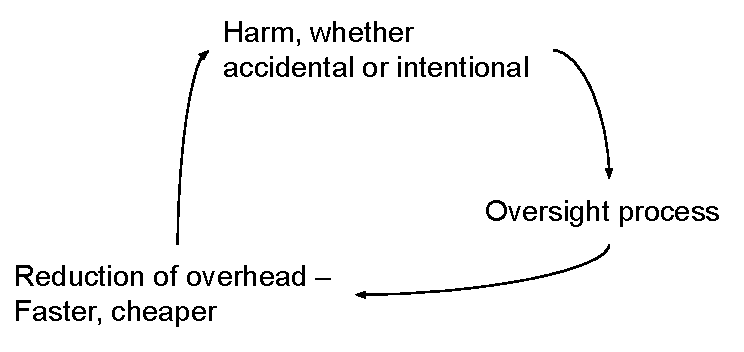
\includegraphics{images/process_loop_harm-oversight-improvement}
    \caption{loop: harm-oversight-improvement}
    \label{fig:harm-oversight-improvement}
\end{figure}


Changing complex processes is hard because individuals involved in the process may depend on steps that are not visible to other people.
Processes do not exist in isolation
\footnote{https://www.hyrumslaw.com/} % https://news.ycombinator.com/item?id=29848295
